\chapter{First steps outside the Local Group of Galaxies:\\
Red Supergiants in NGC\,55}

% \textbf{Completeness:} \textbf{30\%} \\
% The observations for this section are complete and the data reduction is
% currently being optimised.

% \textbf{Description:} \\
% This chapter will outline KMOS observations of 20 RSGs in NGC\,55.
% I will descibe the work I have done in preperation for these observations.

% I will discuss the optimisations which have been made for this data set and
% describe the challenges of obtaining the best possible data from a set of
% challenging observations.

% I will comment on the spatial distribution of the chemical abundances in this
% galaxy and discuss a potential metallicity gradient previously suggested in
% the literature.

\section{Opening remarks} % (fold)
\label{sec:opening_remarks}

Owen has kindly helped reconstruct and combine the data sets

% section opening_remarks (end)

\section{Introduction} % (fold)
\label{sec:introduction}

NGC\,55 is a galaxy located outside of the Local Group of Galaxies potentially within the Sculptor Group at a distance of 1.94\,$\pm$\,0.03\,Mpc~\citep{2006AJ....132.2556P,2008ApJ...672..266G} which, before the emergence of the Araucaria Project~\citep{2005Msngr.121...23G}, been subject to considerable uncertainty~\citep[e.g.]{1987ApJ...323...79P,2006A&A...455..891V}.

The Sculptor Group is considered to be the closest group of galaxies to our own and offers a fantastic laboratory with which to test theories of stellar and galactic evolution.
Association to the Sculptor group however, is a contentious issue.
Distance estimates vary to each galaxy, but typically when one references this group the main galaxies associated to this reference are: NGC\,55, NGC\,247, NGC\,253, NGC\,300 and NGC\,7793.
In addition to these five large spiral galaxies, there are also numerous ($\sim$20) dwarf galaxies associated to this group.

By revising distances for nine of these dwarfs~\cite{2003A&A...404...93K} postulated that the Sculptor group was actually more like a filament of galaxies, which intersects the Milky Way group, where NGC\,55 and NGC\,300 and their surrounding satellite galaxies were potentially not associated with the main group of galaxies in this filament.
Regardless of the geometry and association to the Sculptor Group, NGC\,55 is the nearest large galaxy to the MW group in the direction of the Scultpor Group.

The morphology of NGC\,55 is asymmetric and complicated owing to the high inclination angle measured for this galaxy~\cite[up to 80\textdegree;][]{1986A&A...166...97H,2013MNRAS.434.3511W}.
\cite{1961ApJ...133..405D} classified this galaxy as an LMC-like spiral barred galaxy (SB(s)m) prompting some claims that this galaxy is an edge on analogue of the LMC.
Figure~\ref{fig:ngc55} shows NGC\,55 and its complicated morphology.
In addition, to NGC\,55 being orientated nearly edge on, extending from the disk-bar system there exists many star formation features such as giant H\,\2 regions as well as supergiant filaments and shells which are thought to allow ionising radiation to be transported to the halo where star-formation is currently occuring~\citep{1996AJ....112.2567F}.

The morphology of NGC\,55, as well as its known population of massive hot stars~\citep{2008A&A...485...41C,2012A&A...542A..79C}, points to a recent history of intense star formation.
This is supported by the infrared morphology of NGC\,55 which is dominated by star young forming features~\citep{2004ApJS..154..248E}.

The metal content of NGC\,55 is expected to be LMC-like, which is supported by~\cite{2012A&A...542A..79C} who measured metallicities of blue supergiants using optical VLT spectroscopy.
Using

Even though the hot massive star population of NGC\,55 has been explored,
there currently exists no confirmed RSGs in NGC\,55.
This study represents the first quantititive study of RSGs in NGC\,55 and, by measuring metallicities of this population, will provide a crutial test of the metallicity gradient within this galaxy.




\begin{figure}
 \centering
 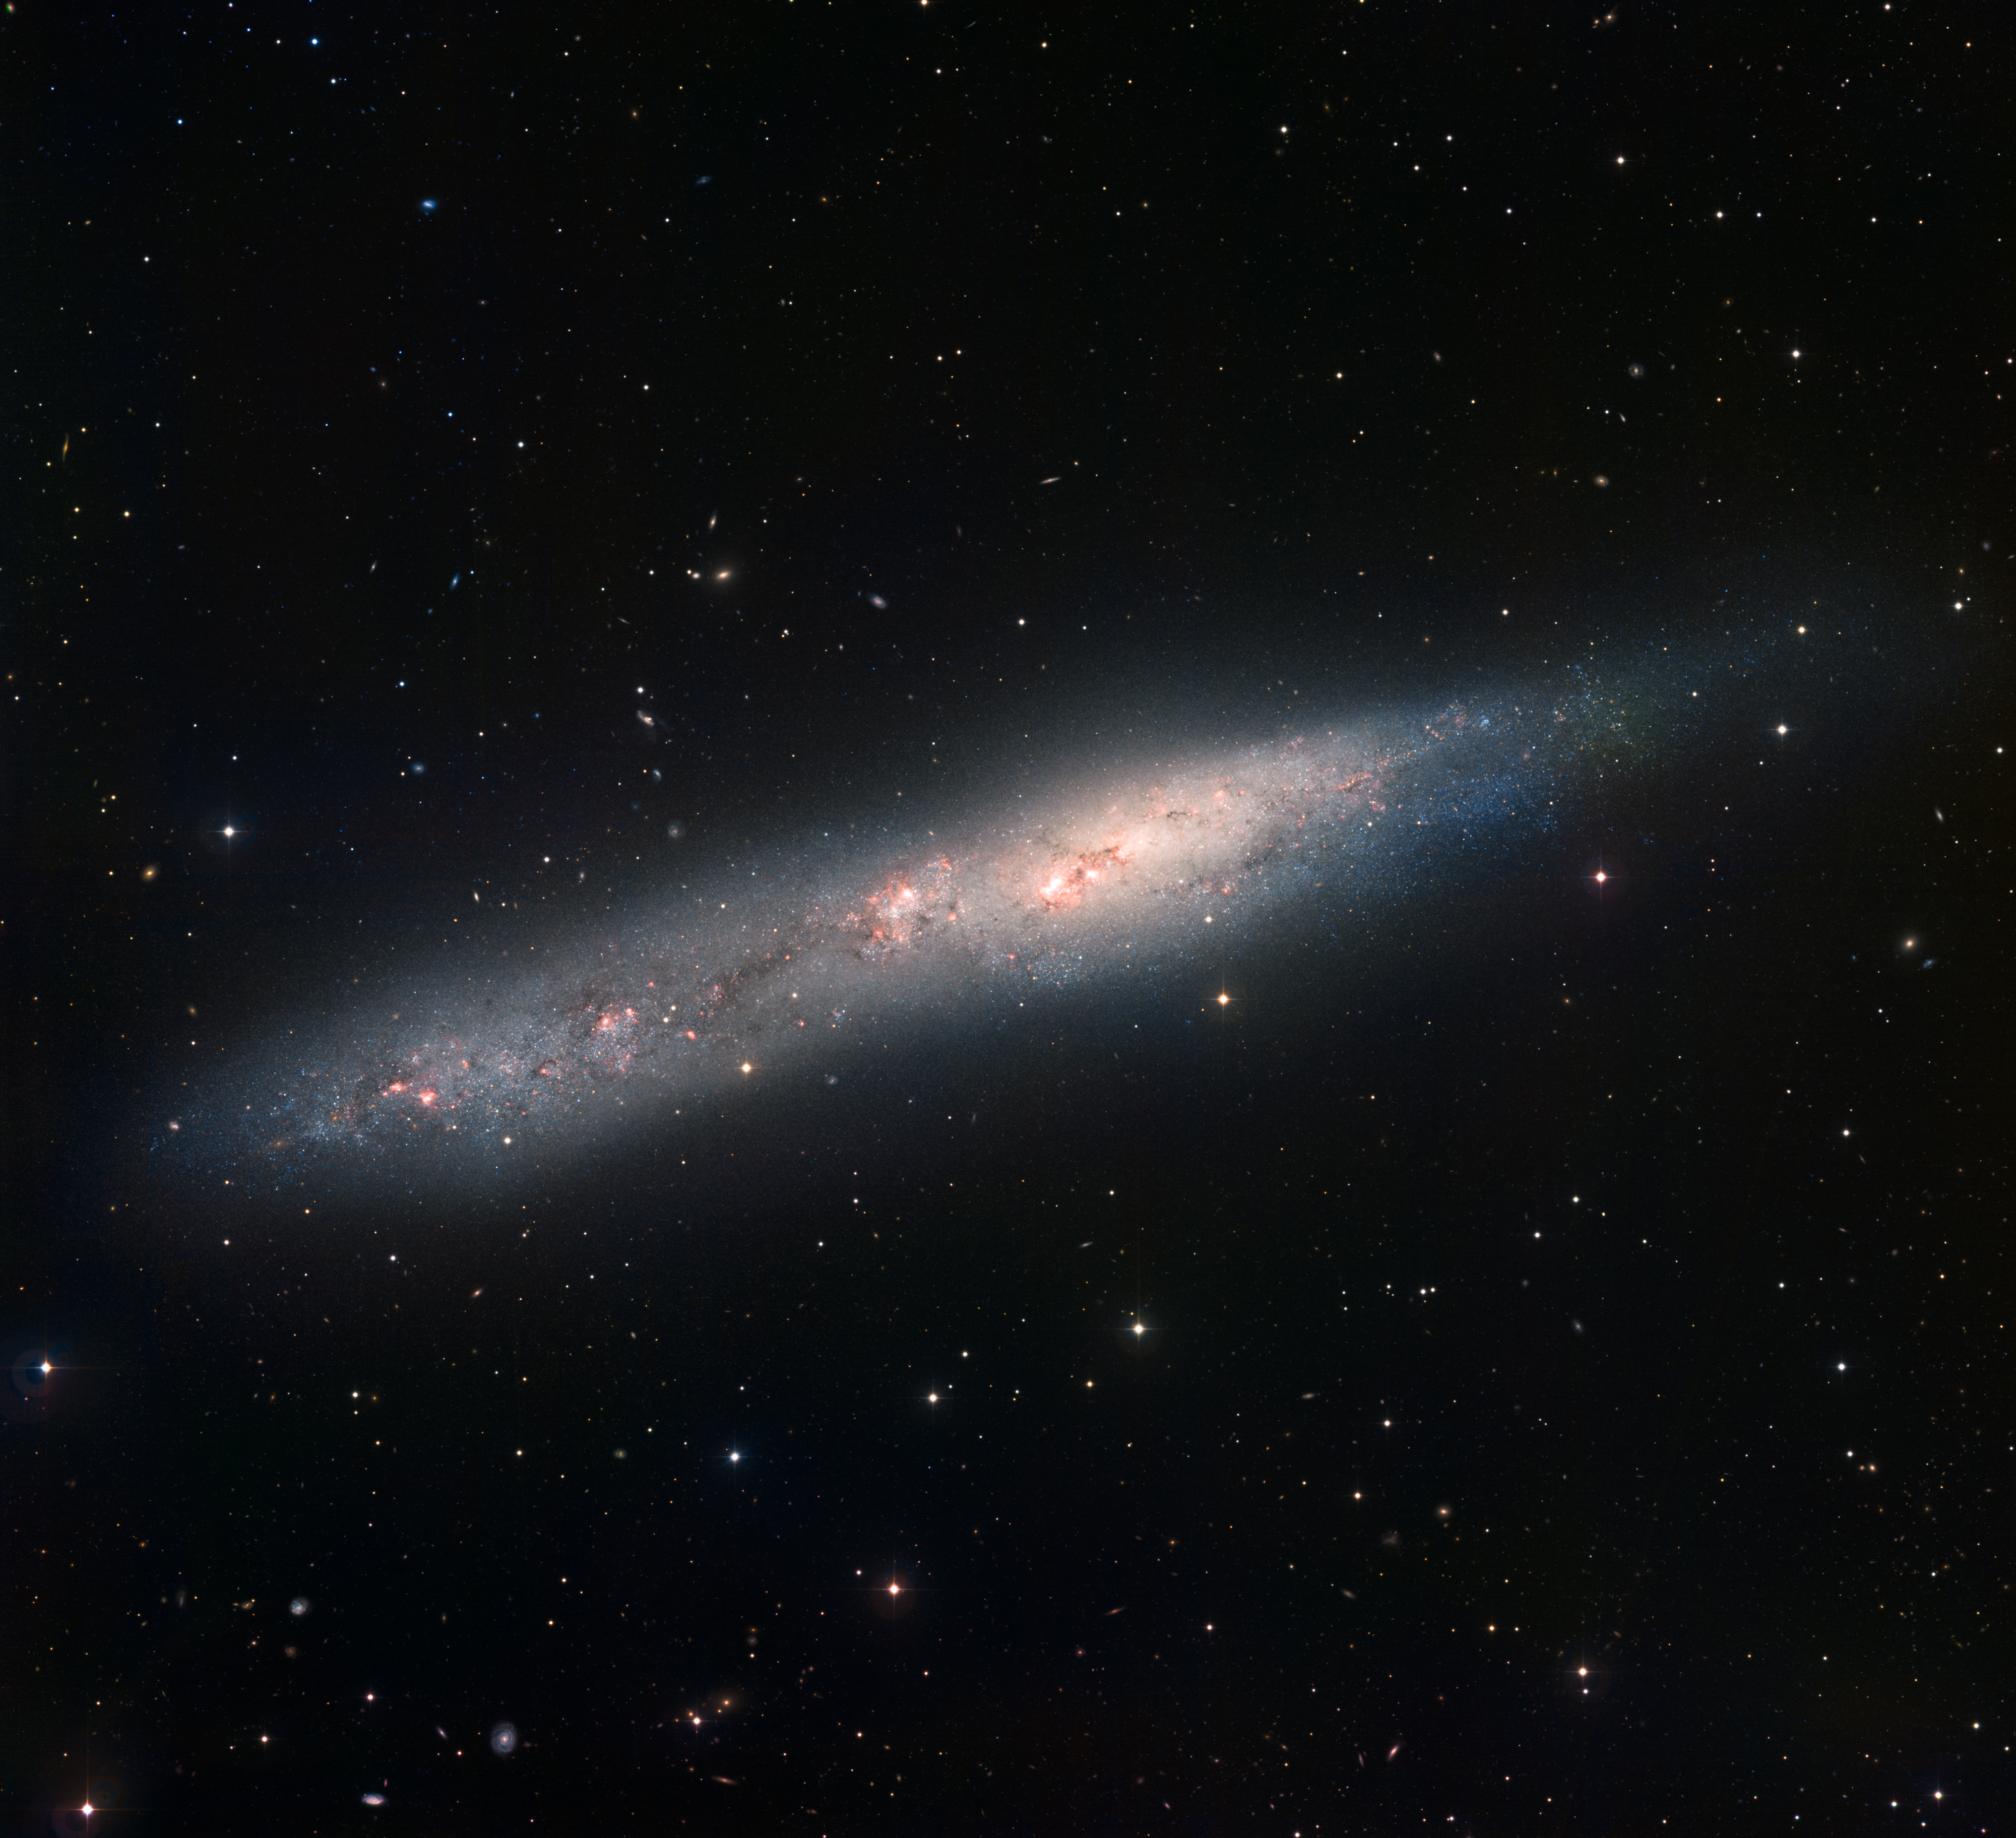
\includegraphics[width=0.65\textwidth]{ngc55/eso0914a}
 \caption[Image of NGC\,55]{Image of NGC\,55 from the Wide Field Imager on the 2.2-metre MPG/ESO telescope at ESO La Silla Observatory. Credit: ESO
 \textbf{Should go the whole hog and bootstrap the RSGs and footprints onto this image ...}}
 \label{fig:ngc55-wide}
\end{figure}


\begin{itemize}
    \item What is NGC\,55?
    \item Why is it important?
    \item What other studies of abundances are present in NGC\,55
    \item Any controvicies? e.g. its distance, association to Sculptor group etc.
\end{itemize}

% section introduction (end)

\section{Observations} % (fold)
\label{sec:observations}

The observations for this study were taken using three nights of KMOS guaranteed time observations (GTO) containing xx RSG candidates, the first of which was taken in October 2013 as part of the observations which led to the publication of~\cite{2015ApJ...805..182G}.
These data consisted of six science exposures (S) of 600\,s with sky offset exposures (S) interleaved in an O, S, O observing pattern.
Seeing conditions for these data were good at 0\farcs8--1\farcs2 throughout the course of the observing block (OB).

The second data set which is made use of in this chapter comes from two nights in September 2014 where the OB used in 2013 was used as backup observations for a programme which required excellent seeing ($<$\,0\farcs6).
The seeing limits on our observations are more relaxed ($<$\,1\farcs5) which gave us an opportunity to make use of some slightly poorer quality KMOS data.
On the first night in September 2014 where this OB was observed, the seeing conditions varied widly ($>$\,1\farcs6) prompting one observer to comment that ``this is the worst recorded seeing at Paranal!''.
However, there are 24 science exposures where the seeing conditions were better than 2\farcs2, which are (potentially) useful.
The final night of observing consisted of 12 exposures with seeing conditions varying between 1\farcs1--1\farcs6.

In addition to the science exposures obtained, on each night a standard set of KMOS calibration files were obtained as well as standard star observations on each night.
The standard star observing block for each night is slightly different where in October 2013 HIP\,3820~\citep[B8\,V;]{1978mcts.book.....H} was observed using the 24-arm telluric template (KMOS\_spec\_acq\_stdstarscipatt).
However, in September 2014 only the three-arm telluric template was observed (KMOS\_spec\_cal\_stdstar), this time with HIP\,18926~\citep[B3\,V;]{1988mcts.book.....H} and HIP\,3820 on both nights.

\textbf{interestingly both with radial velocity measurements. Could do some nice calibration of the RV measurements? or update their measurements ... remember, we've chosen them to be featureless in this region}

Table~\ref{tb:55res} shows the mean measured resolution and resolving power, at the appropriate rotator angles, for each night where the NGC\,55 data were taken.
This table shows that the resolution can vary significant between each night, particularly on detector three where the mean resolving power changes by a factor of 1/5.

\begin{table*}
\caption[Measured velocity resolution for each night]
{Measured velocity resolution and resolving power across each detector.\label{tb:55res}}
\scriptsize
\begin{center}
\begin{tabular}{ccrcccc}
\hline
\hline
Date & Det. & IFUs & \multicolumn{2}{c}{Ne\,\lam1.17700\,$\mu$m}
            & \multicolumn{2}{c}{Ar\,\lam1.21430\,$\mu$m} \\
& & & FWHM (\kms) & $R$ & FWHM (\kms) & $R$ \\
  \hline
  \\
           & 1 & 1-8 &   95.48\,$\pm$\,2.46 & 3140\,$\pm$\,81 &
                         90.78\,$\pm$\,2.12 & 3302\,$\pm$\,77 \\
16-10-2013 & 2 & 9-16 &  88.91\,$\pm$\,1.66 & 3371\,$\pm$\,63 &
                         86.30\,$\pm$\,1.85 & 3473\,$\pm$\,74 \\
           & 3 & 17-24 & 82.96\,$\pm$\,2.14 & 3612\,$\pm$\,76 &
                         80.77\,$\pm$\,2.14 & 3712\,$\pm$\,98 \\
                         \\
\hline
\\
           & 1 & 1-8 &   84.18\,$\pm$\,1.93 & 3561\,$\pm$\,82 &
                         90.78\,$\pm$\,2.12 & 3302\,$\pm$\,77 \\
14-09-2015 & 2 & 9-16 &  87.00\,$\pm$\,1.69 & 3446\,$\pm$\,67 &
                         84.67\,$\pm$\,1.93 & 3541\,$\pm$\,81 \\
           & 3 & 17-24 & 97.14\,$\pm$\,1.88 & 3086\,$\pm$\,60 &
                         94.85\,$\pm$\,2.01 & 3161\,$\pm$\,67 \\
                         \\
\hline
\\
           & 1 & 1-8 &   82.55\,$\pm$\,1.96 & 3632\,$\pm$\,86 &
                         80.41\,$\pm$\,2.30 & 3728\,$\pm$\,106\\
15-09-2014 & 2 & 9-16 &  88.08\,$\pm$\,1.78 & 3404\,$\pm$\,69 &
                         86.03\,$\pm$\,1.96 & 3485\,$\pm$\,80\o\\
           & 3 & 17-24 & 98.04\,$\pm$\,1.91 & 3058\,$\pm$\,59 &
                         96.74\,$\pm$\,2.05 & 3099\,$\pm$\,66\o\\
                         \\
\hline
\end{tabular}
\end{center}
\end{table*}



\subsection{Target Selection} % (fold)
\label{sub:target_selection}
Targets were selected based on the optical photometry from the Araucaria Project~\citep{2005Msngr.121...23G}.
The optical CMD which is used to select targets is displayed in Figure~\ref{fig:VI}, where the RSG candidates are within the grey box and the observed targets are highlighted in red.
This method of target selection was chosen based on the limited extent of near-IR photometry in this area.
Figure~\ref{fig:ngc55} displays the footprints from the Araucaria Project
(green) and the ACS Nearby Galaxy Survey Treasury~\citep[blue; ANGST][]{2009ApJS..183...67D} in NGC\,55 overlaid on a --- image.

The selection criteria employed in this study makes use of the optical $V-I$ colours and $m_I$ magnitudes.
Owing to their cool temperatures and extreme luminosities RSGs are known to exist in a ``plume'' at the tip of a structure of cool stars in the $V-I$, $m_I$ CMD~\citep.
Figure~\ref{fig:VI} displays this CMD and the region of parameter space where RSG candidates reside is marked with a grey box.
This box has the limits $17 < m_I < 19$ and $1.2 < V-I < 3.5$ following~\cite{2015ApJ...805..182G}.
The lower limit of this box are naturally blended in to a population of super-AGB stars which can have luminosities comparable to the faintest RSGs~\citep[e.g.]{2000ApJ...542..804N}.
However, as stated in Chapter~\ref{ch:n6822} these stars are known to have lifetimes similar to the lowest mass RSGs and arguably still trace the young stellar population of this galaxy.

Table~\ref{tb:n55obs-params} shows ground- and space-based optical photometry of the KMOS targets along with their radial velocities (see section~\ref{sub:rvs}).

\begin{figure}
 \centering
 \includegraphics[width=0.65\textwidth]{ngc55/ngc55_V_I}
 \caption[$V-I$ against $V$ colour magnitude diagram for an NGC\,55 field]{
          Colour magnitude diagram for the NGC\,55 optical photometry from the Araucaria Project~\cite{2005Msngr.121...23G}.
          \textbf{placeholder! -- currently this is from the ANGST data}
         }
 \label{fig:VI}
\end{figure}

\begin{figure}
 \centering
 \includegraphics[width=0.65\textwidth]{ngc55/ngc55_fields}
 \caption[Image of NGC\,55 with KMOS targets and photometric footprints highlighted]{
          Image of NGC\,55 with KMOS targets overlaid in red and photometric footprints from the Araucaria Project
          \protect\citep{2005Msngr.121...23G} and the ANGST project
          \protect\citep{2009ApJS..183...67D} highlighed with black shapes.
          \textbf{placeholder! Should do this properly and overlay the regions etc on the pretty eso image.}
         }
 \label{fig:ngc55}
\end{figure}

\begin{sidewaystable}
\caption[Summary of VLT-KMOS targets in NGC\,55]{Summary of VLT-KMOS targets in NGC\,55.\label{tb:n55obs-params}}
\scriptsize
\begin{threeparttable}
\centering
\begin{tabular}{lrcccccccccl}
 \hline
 \hline
ID & S/N & $\alpha$ (J2000) & $\delta$ (J2000) & $V$ & $I$ & $F606$ & $F814$ & \multicolumn{3}{c}{$rv$} (\kms) & Notes \\
& &  & & & & & & 16-10-2013 & 14-09-2014 & 15-09-2014\\

 \hline
NGC55-RSG19 & xx & 00:15:29.190 & $-$39:14:08.20& V & 17.73 & F606 & F814 & RV1 & RV2 & RV3 & Notes\\
NGC55-RSG20 & xx & 00:15:29.520 & $-$39:15:13.00& V & 18.95 & F606 & F814 & RV1 & RV2 & RV3 & Notes\\
NGC55-RSG22 & xx & 00:15:30.520 & $-$39:16:36.70& V & 18.56 & F606 & F814 & RV1 & RV2 & RV3 & Notes\\
NGC55-RSG24 & xx & 00:15:31.460 & $-$39:14:46.30& V & 18.48 & F606 & F814 & RV1 & RV2 & RV3 & Notes\\
NGC55-RSG25 & xx & 00:15:31.490 & $-$39:14:32.40& V & 18.39 & F606 & F814 & RV1 & RV2 & RV3 & Notes\\
NGC55-RSG26 & xx & 00:15:33.160 & $-$39:13:42.00& V & 17.96 & F606 & F814 & RV1 & RV2 & RV3 & Notes\\
NGC55-RSG28 & xx & 00:15:36.160 & $-$39:15:29.40& V & 18.99 & F606 & F814 & RV1 & RV2 & RV3 & Notes\\
NGC55-RSG30 & xx & 00:15:38.030 & $-$39:14:50.20& V & 18.73 & F606 & F814 & RV1 & RV2 & RV3 & Notes\\
NGC55-RSG35 & xx & 00:15:39.260 & $-$39:15:01.70& V & 17.87 & F606 & F814 & RV1 & RV2 & RV3 & Notes\\
NGC55-RSG36 & xx & 00:15:39.520 & $-$39:16:23.10& V & 18.46 & F606 & F814 & RV1 & RV2 & RV3 & Notes\\
NGC55-RSG39 & xx & 00:15:40.260 & $-$39:15:01.00& V & 17.97 & F606 & F814 & RV1 & RV2 & RV3 & Notes\\
NGC55-RSG43 & xx & 00:15:40.700 & $-$39:14:50.20& V & 18.18 & F606 & F814 & RV1 & RV2 & RV3 & Notes\\
NGC55-RSG46 & xx & 00:15:41.640 & $-$39:14:58.80& V & 18.44 & F606 & F814 & RV1 & RV2 & RV3 & Notes\\
NGC55-RSG57 & xx & 00:15:45.590 & $-$39:15:16.40& V & 18.22 & F606 & F814 & RV1 & RV2 & RV3 & Notes\\
NGC55-RSG58 & xx & 00:15:46.270 & $-$39:15:43.20& V & 18.40 & F606 & F814 & RV1 & RV2 & RV3 & Notes\\
NGC55-RSG60 & xx & 00:15:49.180 & $-$39:17:19.80& V & 18.85 & F606 & F814 & RV1 & RV2 & RV3 & Notes\\
NGC55-RSG65 & xx & 00:15:51.250 & $-$39:16:26.40& V & 17.65 & F606 & F814 & RV1 & RV2 & RV3 & Notes\\
NGC55-RSG67 & xx & 00:15:53.110 & $-$39:14:13.60& V & 18.05 & F606 & F814 & RV1 & RV2 & RV3 & Notes\\
NGC55-RSG69 & xx & 00:15:55.280 & $-$39:15:00.10& V & 18.67 & F606 & F814 & RV1 & RV2 & RV3 & Notes\\
NGC55-RSG70 & xx & 00:15:56.310 & $-$39:16:08.60& V & 18.91 & F606 & F814 & RV1 & RV2 & RV3 & Notes\\
NGC55-RSG71 & xx & 00:15:56.900 & $-$39:15:27.50& V & 18.56 & F606 & F814 & RV1 & RV2 & RV3 & Notes\\
NGC55-RSG73 & xx & 00:15:57.710 & $-$39:15:41.50& V & 18.41 & F606 & F814 & RV1 & RV2 & RV3 & Notes\\
\hline
\end{tabular}
\begin{tablenotes}
  \item Ground based data from the Araucaria Project
  \protect\cite{2006AJ....132.2556P}, with typical photometric uncertainty 0.01 and 0.01 in $V$ and $I$ bands respectively.
  Supplementary ANGST data from
  \protect\cite{2009ApJS..183...67D}, with typical errors 0.015, 0.010, 0.012, in $J, H$ and $K$ bands respectively.
\end{tablenotes}
\end{threeparttable}
\end{sidewaystable}

% subsection target_selection (end)

% section observations (end)

\section{Data Reduction} % (fold)
\label{sec:data_reduction}

The data reduction was performed with the KMOS/esorex pipeline with a several corrections to improve the quality of the reductions which are fully described and characterised in~\cite{Turner-prep}.

\begin{itemize}
    \item Split recombined sky frames into seeing bins
    \item combine by including pixel shifts between reconstructed IFUs to ensure all frames are correctly matched
    \item etc.
\end{itemize}

Would it be useful to use Skycorr to subtract the sky as in Gazak et al. (2015)

Telluric correction has been performed by combining and reconstrucitng the telluric standard exposures using the standard pipeline routines.
To improve the performance of the telluric correction I use the method described in detail in Chapter~\ref{ch:n6822}.

As mentioned above, were multiple standard star OBs for each night of observing.
The telluric spectrum used to correct each science spectrum is determined on a star-by-star basis depending upon a visual inspection of the results of the correction.

% section data_reduction (end)

\section{Results} % (fold)
\label{sec:results}

\subsection{Radial Velocities} % (fold)
\label{sub:rvs}
\begin{itemize}
    \item Association with NGC\,55
    \item Does this desrve a subsection of its own?
    \item Radial velocity Vs. Radius from galaxy centre
\end{itemize}
% subsection radial_velocities (end)
\subsection{Stellar Parameters} % (fold)
\label{sub:stellar_parameters}
\begin{itemize}
    \item Comparison to previous results
    \item [Z] Vs. Radius from galaxy centre
    \item MCMC parameter estimation for the fit
    \end{itemize}

% subsection stellar_parameters (end)

% section results (end)

\section{Discussion} % (fold)
\label{sec:discussion}

\begin{itemize}
    \item Orientation of NGC\,55
\end{itemize}
% section discussion (end)

\section{Conclusions} % (fold)
\label{sec:conclusions}

% section conclusions (end)

